%%==================================================
%% chapter01.tex for BIT Master Thesis
%% modified by pinren lu
%% version: 0.1
%% last update: Dec 25th, 2016
%%==================================================
% TOSWT 数据集构建

% 1. 引言
% 2. 方法
%    1. ChatGPT3.5
%    2. GPT4o
%    3. Qwen
%    4. DS
%    5. Gemini
% 3. 数据集介绍
% 4. 本章小结

\chapter{模型改写文本检测数据集构建方法}
\label{chap:TOSWT}

\section{引言}
\label{sec:TOSWT-intro}

在前两章中, 我们详细介绍了探测 AI 生成文本的前世今生。在本章节中,我们将构造出属于自己的数据集。我们的数据集名称叫做追踪学生写作文本来源数据集(Tracing the Origins of Students’ Writing Texts, 以下简称 TOSWT 数据集)在前人的基础上,我们首先要在教育学领域,为教师提供分析文本来源的工具数据集,其次要将数据集更加细粒度,例如探索句子级别,使得实验有着更广泛的应用性,可以帮助教师敏锐地指出学生文本中哪一句经过了什么大型语言模型的修改。

在 Learning Agency Lab 发布的 Automated Essay Scoring 2.0 \cite{learning-agency-lab-automated-essay-scoring-2} (AES2) 数据集的基础上,TOSWT 数据集应运而生。AES2 数据集是一个用于自动写作评价的数据集,包含了 10,584 篇由 9-12 年级学生撰写的短文,并为每篇文章提供了 1-6 分的评分,其中高质量的文本将获得更高的评分。我们在 AES2 数据集的基础上,对原始数据进行了清洗,利用正则表达式替换非 ASCII 字符,并使用句子分割工具将短文划分为句子。此后,我们选用了一种 prompt 进行引导大语言模型改写处理后的短文。

Automated Essay Scoring 2.0 数据集发布于 Kaggle 平台上,为解决自动写作评估问题召开比赛,作为比赛用数据集。短文写作是评估学生学习和表现的重要方法。教育者手工评分也很耗时。自动写作评估(Automated Writing Evaluation, AWE)系统可以对论文进行评分,以补充教育者的其他努力。自动写作评估系统还允许学生定期及时地收到关于他们写作的反馈。但是,由于其成本,该领域的许多进步并没有广泛地提供给学生和教育者。评估学生写作的开源解决方案需要用这些重要的教育工具到达每个社区。

以前开发开源自动写作评估系统的努力受到小型数据集的限制,这些数据集不是广泛性的,也不专注于常见的短文格式。之前在 Kaggle 平台上举办的第一届自动论文评分竞赛对学生写的简短答案进行评分,然而,这是一项课堂上不常使用的写作任务。为了改进以前的努力,需要一个更广泛的数据集,包括高质量、现实的课堂写作样本。此外,为了扩大影响,数据集应该包括跨经济和地点人群的样本,以减轻算法偏见的可能性。

因此 Learning Agency Lab 发布 Automated Essay Scoring 2.0 数据集,这是当时最大的开放获取写作数据集,且该数据集符合当时学生的评估标准。AES2 数据集示例如表 \ref{tab:AES2-example} 所示,其中仅列举 1-3 分数据样例各一个,并省略掉了原文中的换行符“\textbackslash{}n”。

\begin{table*}[htbp]
\caption{AES2 数据集数据示例} \label{tab:AES2-example}
\begin{tabular}{cp{12cm}c}
\toprule
\textbf{essay\_id} & \multicolumn{1}{c}{\textbf{原文}}  & \textbf{评分} \\ \midrule
eb8f967 & Honestly, who would think there   is "Alien Form" on Mars, I mean some of the people are just plain   stupid, and some have facts and details. I think that these so called aliens   are just Fallen Angels, because I read the Bible. These are simply just   natural lanforms. When you take a look at this structure it does look like   a humans face. Then again, I dont think it is an alien monument because, from   how far you look at it and how far they took pictures from it. I don't think   aliens could have made a face a couple miles long, it would have to take   years to do this. Anyhow, I do believe there was life on the planet, I know   there was water, because they have lots of craters, canyons, and   mountains. My conclusion is, they were formed by natural occurances. As in   the passage they compared the face to some features in the American West such   as, Middle Butte, and Snake River Plain of Idaho in the West. These   conlusions matched the face up to natural formation. The face formation is   known as a messa or a plataeu.  & 1  \\ \midrule
7913c3a & My position on driverless cars   is very nutral. Like the passage stated there are a lot pros and cons when it   comes to this topic, such as numerous types of road blocks like accidents and   construction. When it comes to the diverless car getting to an accident   people are confused on who it should be to blame the manufacturer, or the   passenger. I personaly believe the passenger should be to blame, it doesn't   matter how advanced the technology is something is bound to go wrong so you   should always be on alert. When it comes to some of the pros there are   some strong ones. Driving will be a lot safer once a majority of people own a   self driving car. There will be almost no accidents do to texting, falling   asleep at the wheel, and drunk driving. Once we get to the point of almost   everyone owning a self diving car they will most likely be eco-friendly. & 2  \\ \midrule
5d147d6 & Having the new technolgy would   help every teacher and school around the world. By being able to tell how a   student feels the teacher can change the way they would teach the classes or   the way they would a explain a lesson. The computer would tell the teacher   how the students are feeling. It would be valuable to have that type of   technolgy in class room becuase it would make teachers jobs less   complicated. Using the new technology would hellep teacher understand the   students in knowing how they feel whithout having to ask them. "A   classroom computer could recognize when a student is becoming confused or   bored". In this example Dr. Huang explains what the cumputer is able to   do it. By telling how a student is feeling this can help teachers be the   teacher not having to ask every student how they feel. The computer would do   it for the teacher. By having the computer know how the student feels the   teaacher can focus more on exlpaing the lesson better and making it easier to   understand for students to understand. "This could modify the   lesson,like an effective human instuctor" Dr. Huang elpaians that   the computer can change it is teaching the lesson like a teacher would it   also states that it would do it as effective as a human instructor would.   That means having that technolgy would help improve schools teach improve   classes and the way people are being tought. & 3  \\ \bottomrule
\end{tabular}
\end{table*}

在 AES2 数据集中,他们应用如下的评分标准来给学生写作短文打分,分数从低到高是 1 分(最低)到 6 分(最高)。与下面所描述的评分标准一样,每个分数之间的差距(例如 1-2 分、3-4 分、4-5 分)应尽可能相等。具体评分准则如下:

\textbf{6 分}:该类文章展现出清晰且稳定的高水平能力,尽管可能存在一些小错误。典型的文章能就议题有效且深刻地阐述观点,展现出卓越的批判性思维;文章能从原文中选取恰当的例子、理由及其他证据来支撑其观点;文章结构合理、重点突出,展现出清晰的连贯性和流畅的思路推进;文章语言运用娴熟,词汇丰富、准确、恰当,句子结构富有变化;文章在语法、用法和书写规范方面基本没有错误。

\textbf{5 分}:该类文章展现出较为稳定的高水平能力,尽管偶尔会出现错误或质量上的小瑕疵。典型的文章能就议题有效阐述观点,展现出较强的批判性思维;文章通常能选用恰当的例子、理由及其他证据来支撑其观点;文章结构良好、重点明确,展现出连贯性和思路推进;文章语言运用熟练,词汇恰当,句子结构有变化;文章在语法、用法和书写规范方面基本没有错误。

\textbf{4 分}:该类文章展现出足够的能力,尽管在质量上会有起伏。典型的文章能就议题阐述观点,展现出合格的批判性思维;文章能运用足够的例子、理由及其他证据来支撑其观点;文章大致结构合理、重点突出,展现出一定的连贯性和思路推进;文章语言运用能力有所波动,词汇基本恰当,句子结构有一定变化;文章可能存在一些语法、用法和书写规范方面的错误。

\textbf{3 分}:该类文章展现出正在发展的能力,但存在以下一项或多项不足:能就议题阐述观点,有一定批判性思维,但可能表现不稳定,或使用的例子、理由及其他证据不足以支撑观点;文章在结构或重点方面存在局限,或在连贯性和思路推进上有不足;文章语言运用有一定能力,但有时词汇使用较弱、选词不当,和 / 或句子结构缺乏变化或存在问题;文章可能存在语法、用法和书写规范方面的错误累积。

\textbf{2 分}:该类文章展现出的能力较弱,存在以下一项或多项缺陷:对议题的观点模糊或极为有限,批判性思维薄弱;文章提供的例子、理由及其他证据不恰当或不充分,无法支撑观点;文章结构混乱和 / 或重点不明确,或在连贯性和思路推进上存在严重问题;文章语言运用能力极低,词汇量极为有限、选词错误,和 / 或句子结构频繁出现问题;文章存在严重的语法、用法和书写规范错误,在一定程度上影响了意思表达。

\textbf{1 分}:该类文章展现出的能力极低或几乎没有,存在以下一项或多项严重缺陷:无法就议题提出可行的观点,或几乎没有提供证据支撑观点;文章毫无条理、没有重点,导致内容不连贯、逻辑混乱;文章在词汇使用上存在根本性错误,和 / 或句子结构存在严重缺陷;文章存在大量语法、用法或书写规范错误,严重干扰了意思的表达。

\section{问题阐述}
\label{sec:TOSWT-task}

文本来源追踪的任务可以数学化地表述为一个文本分类问题。我们定义一个文本语料库 \( T = \{t_1, t_2, \ldots, t_n\} \),其中每个文本 \( t_i \) 被表示为一个字符串,表示一段文本内容。我们的目标是将每个文本 \( t_i \) 分类到一个预定义的类别集合 \( C = \{c_1, c_2, \ldots, c_k\} \)。

这一过程可以通过以下步骤进行阐述:

1. \textbf{模型训练}:构建一个分类模型 \( f: T \to C \),该模型从训练数据集 $ D = \{(x_1, y_1),\\ (x_2, y_2), \ldots, (x_p, y_p)\} $ 中学习。在这里,\( y_i \in C \) 表示文本 \( t_i \) 的真实类别,而 \( x_i \in T \) 则代表相应的文本内容。模型通过学习这些样本之间的关系,逐渐形成对文本特征和类别之间映射的理解。

2. \textbf{分类过程}:对于新的文本 \( t_{new} \),特征提取过程生成 \( x_{new} \)。随后,利用训练好的模型进行预测:

   \[
   \hat{y} = f(x_{new})
   \]

   其中,\( \hat{y} \) 表示模型预测的类别。这个步骤的核心在于模型能够有效地将新文本映射到其可能的类别中,展现出其在特征空间中的判断能力。

3. \textbf{评估}:模型的性能通过计算一系列评估指标来进行评估,这些指标包括准确率、精确率、召回率和F1分数等。这些指标不仅帮助我们衡量模型在训练集上的表现,还能够评估其在未见数据上的泛化能力,从而确保模型在实际应用中的有效性。

通过上述步骤,我们能够系统地处理文本来源追踪的任务,将其转化为一个可操作的文本分类问题。这一方法论不仅为文本分类提供了清晰的框架,也为后续的研究和应用奠定了坚实的基础。


\section{模型改写文本检测数据集构建}
\label{sec:TOSWT-gen}

在 Learning Agency Lab 发布的 Automated Essay Scoring 2.0 (AES2) 数据集的基础上,TOSWT 数据集应运而生。AES2 数据集是一个用于自动写作评价的数据集,包含了 10,584 篇由 9-12 年级学生撰写的短文,并为每篇文章提供了 1-6 分的评分,其中高质量的文本将获得更高的评分。我们在 AES2 数据集的基础上,对原始数据进行了清洗,利用正则表达式替换非 ASCII 字符,并使用句子分割工具将短文划分为句子。此后,我们选用了一种 prompt 进行引导大语言模型改写处理后的短文。详细过程如图 \ref{fig:dataset-construct} 所示。

\begin{figure*}[htbp]
    \centering
    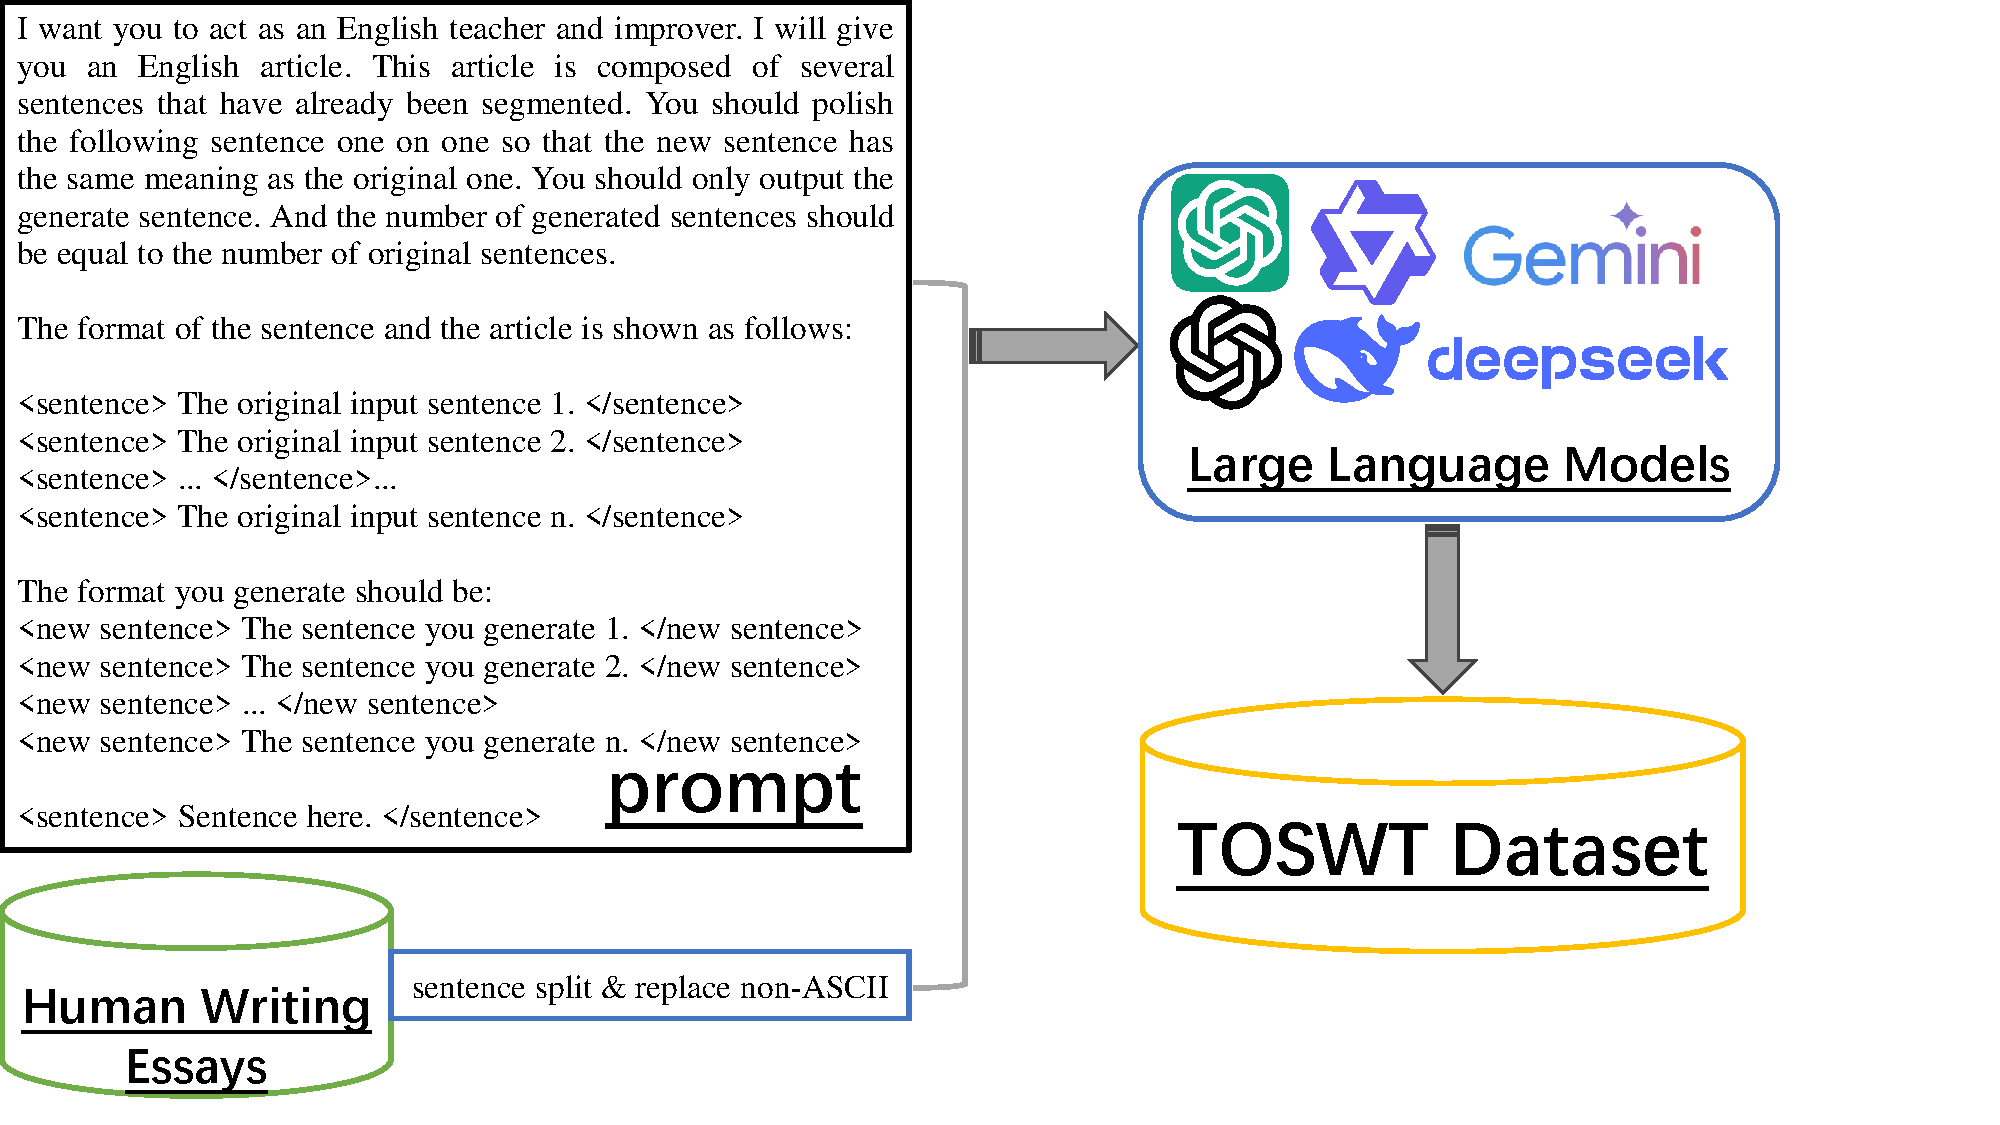
\includegraphics[trim=0 0 150 0, width=\textwidth]{figures/dataset-construct.pdf}
    % TOSWT 数据集构造流程。先将 AES2 中人类写作的短文经过句子分割、将非 ASCII 字符替换后,把每一句嵌入 prompt 中的 <sentence></sentence> 中。
    \caption{TOSWT 数据集的构造过程图}
    \label{fig:dataset-construct}
\end{figure*}

生成 TOSWT 数据集时使用 prompt 翻译表如表 \ref{tab:TOSWT-prompt} 所示。整体分成四个段落,第一段为任务的描述,二、三段则给出输入及输出的格式,最后第四段给予大语言模型输入的句子文本。

这个 prompt 旨在帮助用户提升英语写作能力,具体通过将一篇英语文章进行润色与改进。它设定了用户作为英语教师和改进者的角色,引导用户逐句处理文本,以确保新生成的句子在意义上与原句一致。每个句子都被要求逐一润色,从而增强语言的流畅性和自然度。在执行过程中,用户将接收到一篇由多个已分割句子组成的文章。为了确保生成句子的数量与原句相等,prompt 设定了清晰的输出要求,用户只需专注于生成的新句子而无需担心格式问题。这种简洁的设计使用户能够更高效地进行文本修改。此外,prompt 提供了具体的格式示例,帮助用户理解所需的输出结构。这种结构化的指导不仅提高了工作效率,还确保了生成文本的规范性和一致性,进而为用户提供了系统的学习与实践体验。通过这种方式,用户能够在实际操作中获得更深刻的语言理解与应用能力。

\begin{table*}[htbp]
    \BITSetup{ misc / tabularFontSize = 6}
    \centering
    \caption{Prompt 中英文对照表} \label{tab:TOSWT-prompt}
    \begin{tabular}{@{}p{7.5cm} p{7.5cm}@{}}
        \toprule
        \textbf{英文} & \textbf{中文} \\ \midrule
        I want you to act as a English teacher and improver. & 我希望你充当一名英语教师和改进者。 \\
        I will give you an English article. & 我将给你一篇英语文章。 \\
        This article is composed of several sentences that have already been segmented. & 这篇文章由几个已经被分割的句子组成。 \\
        You should polish the following sentence one on one so that the new sentence has the same meaning as the original one. & 你应该逐句润色以下句子,使新句子与原句具有相同的意思。 \\
        You should only output the generate sentence. & 你只需输出生成的句子。 \\
        And the number of generated sentences should be equal to the number of original sentences. & 生成的句子数量应与原句数量相等。 \\ \midrule
        The format of the sentence and the article is shown as follows: & 句子和文章的格式如下所示: \\
        <sentence> The original input sentence 1. </sentence> & <sentence> 原始输入句子 1。 </sentence> \\
        <sentence> The original input sentence 2. </sentence> & <sentence> 原始输入句子 2。 </sentence> \\
        <sentence> ... </sentence>... & <sentence> ... </sentence>... \\
        <sentence> The original input sentence n. </sentence> & <sentence> 原始输入句子 n。 </sentence> \\ \midrule
        The format you generate should be: & 你生成的格式应为: \\
        <new sentence> The sentence you generate 1. </new sentence> & <new sentence> 你生成的句子 1。 </new sentence> \\
        <new sentence> The sentence you generate 2. </new sentence> & <new sentence> 你生成的句子 2。 </new sentence> \\
        <new sentence> ... </new sentence> & <new sentence> ... </new sentence> \\
        <new sentence> The sentence you generate n. </new sentence> & <new sentence> 你生成的句子 n。 </new sentence> \\ \midrule
        <sentence> Sentence here. </sentence> & <sentence> 句子在这里。 </sentence> \\
        \bottomrule
    \end{tabular}
\end{table*}

\subsection{正则表达式替换非ASCII字符}
\label{sec:TOSWT-gen-reg}

正则表达式替换符号如表 \ref{tab:TOSWT-reg} 所示。在 AES2 数据集以及大型语言模型改写后的文本中均使用正则表达式将非 ASCII 字符替换为相对应的 ASCII 字符,以保证非 ASCII 字符不会影响数据集的效果。

\textbackslash{}u00a0 和 \textbackslash{}u2019 均为 Unicode 编码而非 ASCII 字符,从表中可知,常见的非 ASCII 字符包括空格、左右双引号、左右单引号、字母变体、短划线等。

\begin{table*}[htbp]
    \centering
    \caption{正则表达式替换符号表} \label{tab:TOSWT-reg}
    \begin{tabular}{ccl}
    \toprule
    \textbf{非 ASCII 字符}   & \textbf{替换后字符} & \textbf{含义} \\ \midrule
    \textbackslash{}u00a0 & \              & 空格          \\
    “                     & "              & 左双引号        \\
    ”                     & "              & 右双引号        \\
    ‘                     & '              & 左单引号        \\
    ’                     & '              & 右单引号        \\
    \textbackslash{}u2019 & '              & 单引号         \\
    á                     & a              & a 变体       \\
    ó                     & o              & o 变体        \\
    –                     & -              & 短划线         \\
    —                     & -              & 短划线2        \\
    …                     & ...            & 一个字符表示三个句号  \\
    é                     & e              & e 变体         \\ \bottomrule
    \end{tabular}
\end{table*}

\subsection{细粒度分割获取句子}
\label{sec:TOSWT-gen-sentence_splitter}

在构建 TOSWT 数据集的过程中,为了使用尽可能细粒度的数据进行训练,因此使用到了句子分割的技术。我们使用的句子分割技术主要参考了 GitHub 上 mediacloud 使用的句子分割技术 \cite{sentence-splitter},并添加了一些修改。

这个句子分割方法的主要功能是将输入的文本字符串分割成单独的句子,并返回一个字符串列表。它通过一系列正则表达式和逻辑规则来识别句子的边界,处理复杂的标点符号和特殊情况。以下是该方法的详细解析:

1. \textbf{输入验证}:首先,函数检查输入的文本是否为 None 或空字符串。如果是 None,会发出一个警告(SentenceSplitterWarning),并返回一个空列表。如果是空字符串,则直接返回空列表。这些检查确保了函数能够优雅地处理无效输入。

2. \textbf{添加句子分隔符}:函数使用多个正则表达式(通过 regex.sub 函数)来识别句子的边界,并在适当的位置插入换行符(\textbackslash{}n)作为分隔符,具体插入规则包括以下四种情况:
(1)非句号的句子结束标记(如 ? 或 !)后面跟随句子开头的标志(如大写字母)。
(2)多重句号(如 ...)后面跟随句子开头的标志。
(3)标点符号后紧跟引号或括号的情况。
(4)句子结束标点后紧跟句子开头标志的情况。

这些规则通过正则表达式的模式匹配来实现,确保了对复杂标点符号的处理。

3. \textbf{特殊标点处理}:在处理完主要的句子分隔符后,函数进一步处理特殊标点符号的情况。它将文本拆分为单词列表,并逐一检查每个单词是否符合特定的模式:
(1)检查是否是已知的荣誉称谓(如 Dr. 或 Mr.),这些通常不会作为句子结束。
(2)检查是否是大写字母缩写(如 U.S.A.),这些也不应被分割。
(3)检查是否是数字相关的非分隔符情况。

通过这些检查,函数能够避免错误地将某些标点符号识别为句子边界。

4. \textbf{清理和返回结果}:在完成所有分隔符的插入后,函数会清理文本中的多余空格和换行符,确保输出的格式整洁。最后,它通过换行符(\textbackslash{}n)将文本分割成句子列表,并返回结果。

本句子分割的设计非常全面,能够处理多种复杂的句子分隔情况,包括标点符号、引号、括号和缩写等。它适用于需要高精度文本分割的场景,如自然语言处理(NLP)任务或文本分析工具。

\subsection{大型语言模型改写文本}
\label{sec:TOSWT-gen-llm}

在经过使用正则表达式替换非 ASCII 字符以及使用 Sentence Splitter 做句子分割后,我们将得到的句子与上表 \ref{tab:TOSWT-prompt} 提及的 Prompt 组合起来丢给大型语言模型进行重写润色。其中,大型语言模型共计五种,其中包括了:ChatGPT(GPT3.5)、GPT4o、Gemini、Qwen 和 DeepSeek。大型语言模型使用模型版本及价格如表 \ref{tab:TOSWT-llmcost} 所示。均选用了较为先进的模型,且可知国内模型如通义千问和 DeepSeek 模型,其价格远低于国外相同类型的模型。

\begin{table*}[htbp]
\centering
\caption{大型语言模型使用版本及定价(2025年4月8日价格)} \label{tab:TOSWT-llmcost}
\begin{tabular}{llcc}
\toprule
\textbf{模型类别} & \textbf{模型版本}                 & \textbf{输入价格}  & \textbf{输出价格}  \\ \midrule
ChatGPT \cite{chatgpt}       & gpt-3.5-turbo-0613            & \$1.5/1M token  & \$2/1M token    \\
GPT4o \cite{gpt4o}         & gpt-4o-2024-08-06             & \$2.5/1M token  & \$10/1M token   \\
Gemini \cite{geminiteam2024geminifamilyhighlycapable}        & gemini-exp-1206               & \$3.5/1M token  & \$14/1M token   \\
Qwen \cite{qwen2025qwen25technicalreport}          & qwen-plus-2024-12-20          & \textyen 0.8/1M token  & \textyen 2/1M token    \\
DeepSeek \cite{deepseekai2024deepseekv3technicalreport}      & deepseek-chat V3 (2024-12-24) & \$0.27/1M token & \$1.10/1M token \\ \bottomrule
\end{tabular}
\end{table*}

这五种大型语言模型在按照提示生成句子时有一定的失败概率,在第一次生成期间成功率如表 \ref {tab:construct-dataset-success-rate} 所示。由于网络波动等相关因素,生成的数据实例总数并不完全一致。Qwen、Gemini和 DeepSeek V3 展示了遵循 Prompt 生成符合格式内容的强大能力。

\begin{table*}[htbp]
    \centering
    % 大语言模型首次生成时遵从 prompt 生成符合格式内容的成功率。
    \caption{大语言模型首次生成时遵从 prompt 生成符合格式内容的成功率}
    \begin{tabular}{l|ccc}
\toprule
\textbf{模型名称} & \textbf{成功个数} & \textbf{生成总数} & \textbf{成功率} \\
\midrule
GPT3.5 \cite{chatgpt}   & 7642      & 10745   & 71.12 \\
GPT4o \cite{gpt4o}   & 8687      & 10745   & 80.85 \\
Gemini \cite{geminiteam2024geminifamilyhighlycapable}  & 9695      & 10745   & 90.23 \\
Qwen \cite{qwen2025qwen25technicalreport}    & 9840      & 10745   & \textbf{91.58} \\
Deepseek \cite{deepseekai2024deepseekv3technicalreport} & 9448      & 10330   & 87.93 \\
\bottomrule
    \end{tabular}
    \label{tab:construct-dataset-success-rate}
\end{table*}

\subsubsection{ChatGPT}
\label{sec:TOSWT-gen-chatgpt}

最早推出的 ChatGPT \cite{chatgpt},也被称为 GPT-3.5(Generative Pre-trained Transformer 3.5),是 OpenAI 在 GPT-3 的基础上进行优化而构建的大型语言模型(LLM)。该模型属于生成式预训练模型家族,基于 Transformer 架构,展现出在自然语言生成(NLG)、理解(NLU)以及多任务处理等方面的卓越性能,广泛应用于学术写作、代码生成和智能客服等多个领域。

ChatGPT 基于 Transformer 架构的神经网络设计,其核心特征在于自注意力机制(Self-Attention)的应用。这一机制能够有效捕捉文本序列中的长距离依赖关系,并支持并行计算,从而提高训练效率。研究表明,该模型的某些版本参数规模可达 1750 亿,通过构建深层网络结构并结合海量训练数据(包括互联网公开文本和学术文献等),显著提升了模型的性能表现。在训练方法上,ChatGPT 采用了“预训练与微调”的混合范式:首先通过无监督学习从大规模语料库中提取通用语言表征,随后结合有监督微调技术进行任务适配。此外,该模型创新性地引入了人类反馈强化学习 \cite{kaufmann2024surveyreinforcementlearninghuman}(Reinforcement Learning from Human Feedback, RLHF)方法,从而有效优化模型输出与人类价值观之间的对齐性。

ChatGPT(GPT-3.5)作为 OpenAI 首个面向公众的大规模对话式人工智能,具有里程碑式的技术发展意义。其历史贡献主要体现在三个方面:首先,它通过免费交互的形式使得具有 1750 亿参数的大型模型能力得以普及,用户在短短两个月内突破一亿,成为历史上增长最快的消费级应用;其次,借助于指令微调和人类反馈强化学习(RLHF)的技术创新,显著增强了模型对人类意图的对齐能力,为后续对话模型的训练框架奠定了基础;最后,其在代码生成、教育辅助等领域的跨领域应用展示了通用人工智能的潜力,例如成功通过美国律师考试并催生了 AIGC 产业生态。然而,随着后续模型(如 GPT-4 和 GPT-4o)的推出,其局限性逐渐显现:上下文窗口仅为 3000 词(而 GPT-4 可达 2.5 万词),在复杂推理和数学计算方面的准确率低于 GPT-4(例如在 LSAT 考试中,GPT-4 的得分高出 15\%);此外,其仅支持文本交互,缺乏多模态能力;知识的时效性受限于 2021 年的训练数据,且幻觉控制能力较弱,事实错误率比 GPT-4 高出约 40\%。这些不足促使模型向更大参数规模、更优对齐性及更低推理成本的方向不断演进。

从技术迭代的角度来看,GPT-3.5 的突破性在于首次验证了大规模预训练模型与人类反馈相结合的优化方案的可行性。然而,其单模态架构及有限的推理能力在专业领域的应用中逐渐显得不足。例如,OpenAI 推出的新一代模型 GPT-4 通过引入多模态处理和万亿级参数,在医学诊断、法律分析等任务中展现出更高的可靠性。而 GPT-4o 则进一步整合了音频和视频交互能力,实现了更为自然的人机交互体验。

\subsubsection{GPT4o}
\label{sec:TOSWT-gen-gpt4o}

GPT-4o \cite{gpt4o} 是 OpenAI 于 2024 年 5 月推出的下一代多模态大语言模型,其中的 "o" 代表 "omni"(全能),标志着其在文本、音频和视觉模态的端到端处理能力上取得了显著突破。该模型采用统一的 Transformer 架构,能够通过单一神经网络直接处理多模态输入(包括文本、图像和音频的任意组合),并生成文本、音频和图像输出的任意组合,从而消除了传统多模态系统中不同模型间转换所带来的延迟问题。GPT-4o 实现了跨文本、视觉和音频的端到端训练,意味着所有输入和输出均由同一神经网络处理。在技术层面,该模型通过改进的词元化(tokenization)方法,将音频特征和视频帧序列编码为与文本相同的表示形式,并利用多头注意力机制实现跨模态的语义关联,能够在低至 232 毫秒的时间内响应音频输入,平均响应时间为 320 毫秒,这与人类在对话中的反应时间相当。

与前代模型相比,GPT-4o 展现出三方面显著优势:首先,其多模态能力实现了质的飞跃,能够执行如图像内容分析生成食谱以及通过呼吸声识别情绪状态等复杂任务;其次,其非英语语言处理能力显著提升,支持 50 种语言的实时翻译,尤其在非拉丁语系文字(如韩语和阿拉伯语)的识别准确率提高超过 20\%;最后,其运行效率得到了显著优化,API 成本较 GPT-4 Turbo 降低了 50\%,推理速度提升了两倍。

\subsubsection{Gemini}
\label{sec:TOSWT-gen-gemini}

Gemini \cite{geminiteam2024geminifamilyhighlycapable} 是 Google DeepMind 开发的一系列多模态大语言模型,标志着谷歌在通用人工智能领域的重要进展。该系列模型于 2023 年 12 月正式推出,其核心创新在于采用原生多模态架构,能够同时处理文本、图像、音频、视频及代码五种信息类型。与传统多模态模型不同,Gemini 从预训练阶段起便利用统一的神经网络处理多模态输入,通过改进的词元化(tokenization)方法将不同模态的数据编码为统一表示,并通过多头注意力机制实现跨模态的语义关联。这一设计使其在复杂推理任务中表现卓越,例如能够理解手写的物理题解答并指出错误推理步骤,或将视觉信息转化为编程代码。在技术层面,Gemini 采用 TPUv4/v5e 加速器进行训练,其训练数据涵盖网络文档、学术文献和多语言语料,并通过人类反馈强化学习 \cite{kaufmann2024surveyreinforcementlearninghuman} (RLHF)优化输出的一致性。

尽管 Gemini 在多模态理解和复杂推理方面展现出优势,但仍存在一定的局限性。早期版本受到质疑,认为其测试分数夸大且演示视频存在剪辑问题,此外在非英语任务中的性能相对较弱。与后续模型相比,Gemini 缺乏动态更新机制,其在专业领域(如医学和法律)的微调效果有待提升。这些不足促使谷歌朝着更大参数规模、更低推理成本和更专业化的方向迭代,例如发布了开源模型 Gemma(20 亿/70 亿参数)。总体而言,Gemini 系列通过原生多模态架构和规模化训练基础设施,为通用人工智能的发展提供了重要的技术范式。

\subsubsection{Qwen}
\label{sec:TOSWT-gen-qwen}

通义千问 \cite{qwen2025qwen25technicalreport}(Qwen)是阿里云自主研发的一系列超大规模语言模型,作为中国人工智能领域的重要代表,其技术进步和产业应用充分体现了国产大模型的发展历程。该模型系列于 2023 年 4 月 11 日正式发布,其名称蕴含双重含义:“通义”象征着模型在跨领域知识理解方面的广泛适用性,而“千问”则源自中国古代百科全书《千问》,彰显其处理复杂问题的能力。在技术架构方面,通义千问采用了改进的 Transformer 结构,通过旋转位置编码 \cite{su2023roformerenhancedtransformerrotary}(RoPE)增强了对长序列的建模能力。此外,该模型创新性地结合了非绑定式嵌入(un-tied embeddings)与 RMSNorm 层进行优化,使其在 72B 参数版本中实现了 2048 个词元的上下文窗口支持。值得一提的是,其开源模型 Qwen1.5-110B 采用了稀疏专家混合(MoE)架构,并在 2024 年 5 月发布的 2.5 版本中,逻辑推理和代码能力较前一代提升了 16\% 和 10\%。

该模型的核心竞争力体现在三个主要方面:多模态融合、产业适配性以及开源生态系统的构建。在模态支持方面,通义千问2.0 已实现对文本、图像和音频的端到端处理,其多模态理解能力使其能够执行从商品设计草图生成营销文案等复杂任务。在产业应用方面,阿里云通过实施“云智一体”战略,将模型能力深度嵌入电商、医疗和金融等多个场景。例如,通义灵码智能编程助手能够完成 85\% 的常规代码生成任务,从而显著提升开发效率。在开源策略方面,截至 2025 年,通义千问已发布从 1.8B 到 110B 参数的七款开源模型,累计下载量超过 700 万次。其中,Qwen-72B 在 MMLU 基准测试中达到了与 Llama3-70B 相当的精度。

与同期国际模型相比,通义千问展现出显著的差异化特征。其训练数据中包含超过 30\% 的高质量中文语料,使其在古文解析和中文创意写作等任务上表现优于同等规模的 GPT-3.5 模型。在商业应用方面,通过实施 API 价格策略(2 元/1M tokens)及轻量化部署方案(例如与联发科天玑9300芯片的适配),显著降低了企业的使用门槛。然而,该模型在处理非拉丁语系的多语言任务时,其准确率仍比 GPT-4 低约 15\%。这些技术优势使通义千问成为中国大模型技术自主创新与全球竞争的重要案例,其发展路径为学术界在 AI 技术产业化方面的研究提供了典型的参考样本。

\subsubsection{DeepSeek}
\label{sec:TOSWT-gen-ds}

DeepSeek V3 \cite{deepseekai2024deepseekv3technicalreport} 是中国深度求索公司(DeepSeek)于2024年12月发布的新一代多模态大语言模型,标志着国产大模型在技术创新与成本控制方面的重要里程碑。该模型采用混合专家(MoE)架构,总参数量达到6710亿,其中每个词元激活370亿参数,通过动态路由机制实现计算资源的高效分配。在技术层面,DeepSeek V3 创新性地结合了多头潜在注意力机制(MLA)与 FP8 混合精度训练。前者通过低秩压缩键值对有效降低内存占用,后者则在矩阵乘法等计算密集型操作中采用 FP8 格式,使得训练成本控制在557.6万美元,仅为 GPT-4o 等主流模型的十分之一。在14.8万亿 token 的预训练基础上,模型通过监督微调和强化学习进一步优化性能,其生成速度达到60 TPS(每秒事务处理量),较前代 V2.5 提升了三倍,显著改善了交互的流畅性。

在性能表现方面,DeepSeek V3 展现出在多个领域的竞争优势。在知识类任务(如 MMLU 和 GPQA)中,其表现接近于 Claude-3.5-Sonnet,而在数学竞赛(如 AIME 2024 和 CNMO 2024)中,其成绩超越了所有开源和闭源模型。此外,其代码生成能力可与 85\% 的人类编程选手相媲美。特别是在中文处理方面,凭借 30\% 的高质量中文语料进行训练,该模型在古文解析和创意写作等任务中优于同等规模的国际模型。2025年3月发布的 V3-0324 版本进一步增强了前端开发能力,能够根据单一提示自动生成包含交互控件和赛博朋克风格界面的完整网站,开发者将其誉为“编码领域的标杆”。该模型支持 128K 的上下文窗口(开源版),在长文本理解任务(如 DROP 和 LongBench v2)中的平均表现领先于行业标准。

DeepSeek V3 的商业化与开源策略是其另一显著特色。其 API 定价极具竞争力,输入和输出词元的成本分别为每百万词元 0.27 美元和 1.10 美元,较国际同类产品降低超过 50\%。该模型采用 MIT 开源协议,允许商业用途及二次开发,截至 2025 年,已实现 700 万次下载,促进了 AI 技术在边缘设备上的部署。其应用场景涵盖智能编程(如通义灵码助手)、金融风险控制及教育辅导等多个领域。在电商平台的数据分析场景中,该模型能够实时识别欺诈交易并生成可视化报告。

尽管 DeepSeek V3 的表现十分出色,但其仍存在一定局限性,尤其是在处理复杂音频和视觉输入时,其幻觉率比文本模态高出约 20\%。然而,DeepSeek V3 现有的诸多优势特性使其成为研究 AI 技术普惠化与计算效率优化的典型案例,为中国大模型在全球竞争中的发展提供了重要参考。

\section{模型改写文本检测数据集}
\label{sec:TOSWT-info}

经过上述大型语言模型的润色,原始的人类写作散文与其改进版本共同构成了模型改写文本检测数据集,总计包含 53,328 篇短文和 147,976 个句子。

新数据集中每篇短文的句子数、每篇散文的词元数以及每个句子的词元数如表 \ref{tab:TOSWT-length} 所示。第一行表示一篇短文中的句子个数,接下来分别是短文与句子的词元个数。50\% 表示的是中位数,其他以此类推。大语言模型的改写倾向于将文本长度改短,使之更加精炼。

\begin{table*}[htb]
\centering
% TOSWT 数据集句子个数及 token 个数。

\caption{模型改写文本检测数据集数据集句子个数及词元个数}
\begin{tabular}{c|l|cccccccc}
\toprule
                          & \textbf{模型}  & \textbf{MIN} & \textbf{10\%} & \textbf{25\%} & \textbf{50\%} & \textbf{75\%} & \textbf{90\%} & \textbf{MAX}  & \textbf{AVG}   \\
    \midrule
                          & 句子个数        & 2   & 8    & 11   & 16   & 21   & 26   & 53   & 16.65  \\ \midrule
\multirow{6}{*}{短文词元} & AES2 \cite{learning-agency-lab-automated-essay-scoring-2}           & 156 & 212  & 267  & 362  & 473  & 588  & 1338 & 385.41 \\
                          & GPT3.5 \cite{chatgpt}         & 84  & 208  & 259  & 349  & 454  & 558  & 1257 & 370.24 \\
                          & GPT4o \cite{gpt4o}          & 122 & 199  & 247  & 331  & 428  & 525  & 1185 & 349.90 \\
                          & Gemini \cite{geminiteam2024geminifamilyhighlycapable}         & 128 & 209  & 261  & 351  & 458  & 565  & 1268 & 372.92 \\
                          & Qwen \cite{qwen2025qwen25technicalreport}           & 111 & 197  & 245  & 325  & 419  & 510  & 1092 & 343.22 \\
                          & Deepseek \cite{deepseekai2024deepseekv3technicalreport}       & 115 & 200  & 249  & 333  & 427  & 517  & 1193 & 349.14 \\
                          \midrule
\multirow{6}{*}{单句词元} & AES2 \cite{learning-agency-lab-automated-essay-scoring-2}           & 4   & 11   & 15   & 20   & 28   & 38   & 305  & 23.15  \\
                          & GPT3.5 \cite{chatgpt}         & 2   & 11   & 15   & 20   & 27   & 35   & 229  & 22.24  \\
                          & GPT4o \cite{gpt4o}          & 2   & 11   & 14   & 19   & 25   & 33   & 257  & 21.02  \\
                          & Gemini \cite{geminiteam2024geminifamilyhighlycapable}         & 4   & 11   & 15   & 20   & 27   & 36   & 308  & 22.40  \\
                          & Qwen \cite{qwen2025qwen25technicalreport}           & 4   & 11   & 14   & 19   & 25   & 32   & 189  & 20.62  \\
                          & Deepseek \cite{deepseekai2024deepseekv3technicalreport}       & 4   & 11   & 14   & 19   & 25   & 33   & 243  & 20.97 \\
                          \bottomrule
\end{tabular}

\label{tab:TOSWT-length}

\end{table*}

\section{本章小结}
\label{sec:TOSWT-conclusion}

本章详细探讨了模型改写文本检测数据集(TOSWT 数据集)的构建方法,旨在为教育工作者提供一个有效的工具,以分析和追踪学生文本的来源。我们从教育学领域的背景出发,强调了构建该数据集的重要性,尤其是在当前人工智能生成文本日益普及的背景下,教师需要具备识别和分析学生写作中可能受到大型语言模型影响的能力。

在数据集的构建过程中,我们以 Learning Agency Lab 发布的 Automated Essay Scoring 2.0 (AES2) 数据集为基础,首先对原始数据进行了系统的清洗和处理。通过使用正则表达式,我们成功替换了非 ASCII 字符,确保了数据的统一性和规范性。这一步骤为后续的分析提供了可靠的基础。

接下来,我们采用了句子分割技术,以实现对文本的细粒度处理。这一技术借助了先进的正则表达式和逻辑规则,能够有效识别句子的边界,处理复杂的标点符号和特殊情况。这种细分方法不仅提高了数据的可用性,还为后续的分析和模型训练奠定了基础。

在生成模型改写文本检测数据集的过程中,我们引入了多种大型语言模型,包括 ChatGPT、GPT4o、Gemini、Qwen 和 DeepSeek。这些模型在文本改写过程中展现出强大的能力,能够将原始文本进行润色和改写,同时保持其原意。通过对比不同模型的表现,我们能够评估其在文本生成任务中的有效性和可靠性。最终,构建出的数据集包含 53,328 篇短文和 147,976 个句子,为后续的文本检测研究提供了丰富的数据支持。

此外,本章还深入探讨了文本来源追踪的数学化表述,将其视为一个文本分类问题。我们详细描述了模型训练的过程,包括数据集的构建、特征提取和模型评估。通过构建一个分类模型,我们能够有效地将新文本映射到预定义的类别中,从而实现对文本来源的追踪和分析。这一方法论为后续研究提供了清晰的框架,确保了文本检测任务的系统性和可操作性。

综上所述,本章的工作不仅为学生写作的文本分析提供了重要的数据支持,也为教师在识别和评估学生写作能力方面提供了有力的工具。通过构建模型改写文本检测数据集,我们为教育领域在人工智能生成文本背景下的研究提供了新的视角和方法,推动了文本来源追踪技术的发展。